\documentclass[11pt]{article}
\usepackage[margin=0.75in]{geometry}
\usepackage{tikz}
\usetikzlibrary{positioning,arrows.meta,calc}
\usepackage{booktabs}
\usepackage{array}
\usepackage{hyperref}
\begin{document}

\begin{center}
{\Large \textbf{Replication-oriented study selection trace}}\\[4pt]
{\small Demonstration diagram for the replication package}
\end{center}

\noindent\textbf{Note.} For the sake of replication and package size, the record-level demonstration in this replication package is centered on the \textbf{802 studies} retained after title/abstract screening, because these are the records for which step-by-step screening decisions are demonstrated in the CSV files. However, \textbf{802 is only the demonstration subset}. The \textbf{actual study flow in the paper} starts from \textbf{4,010 initial records} and ends with \textbf{107 final primary studies}. Both the full-study summary flow and the 802-record demonstration trace are preserved in this package.

\begin{figure}[h!]
\centering
\resizebox{0.96\textwidth}{!}{%
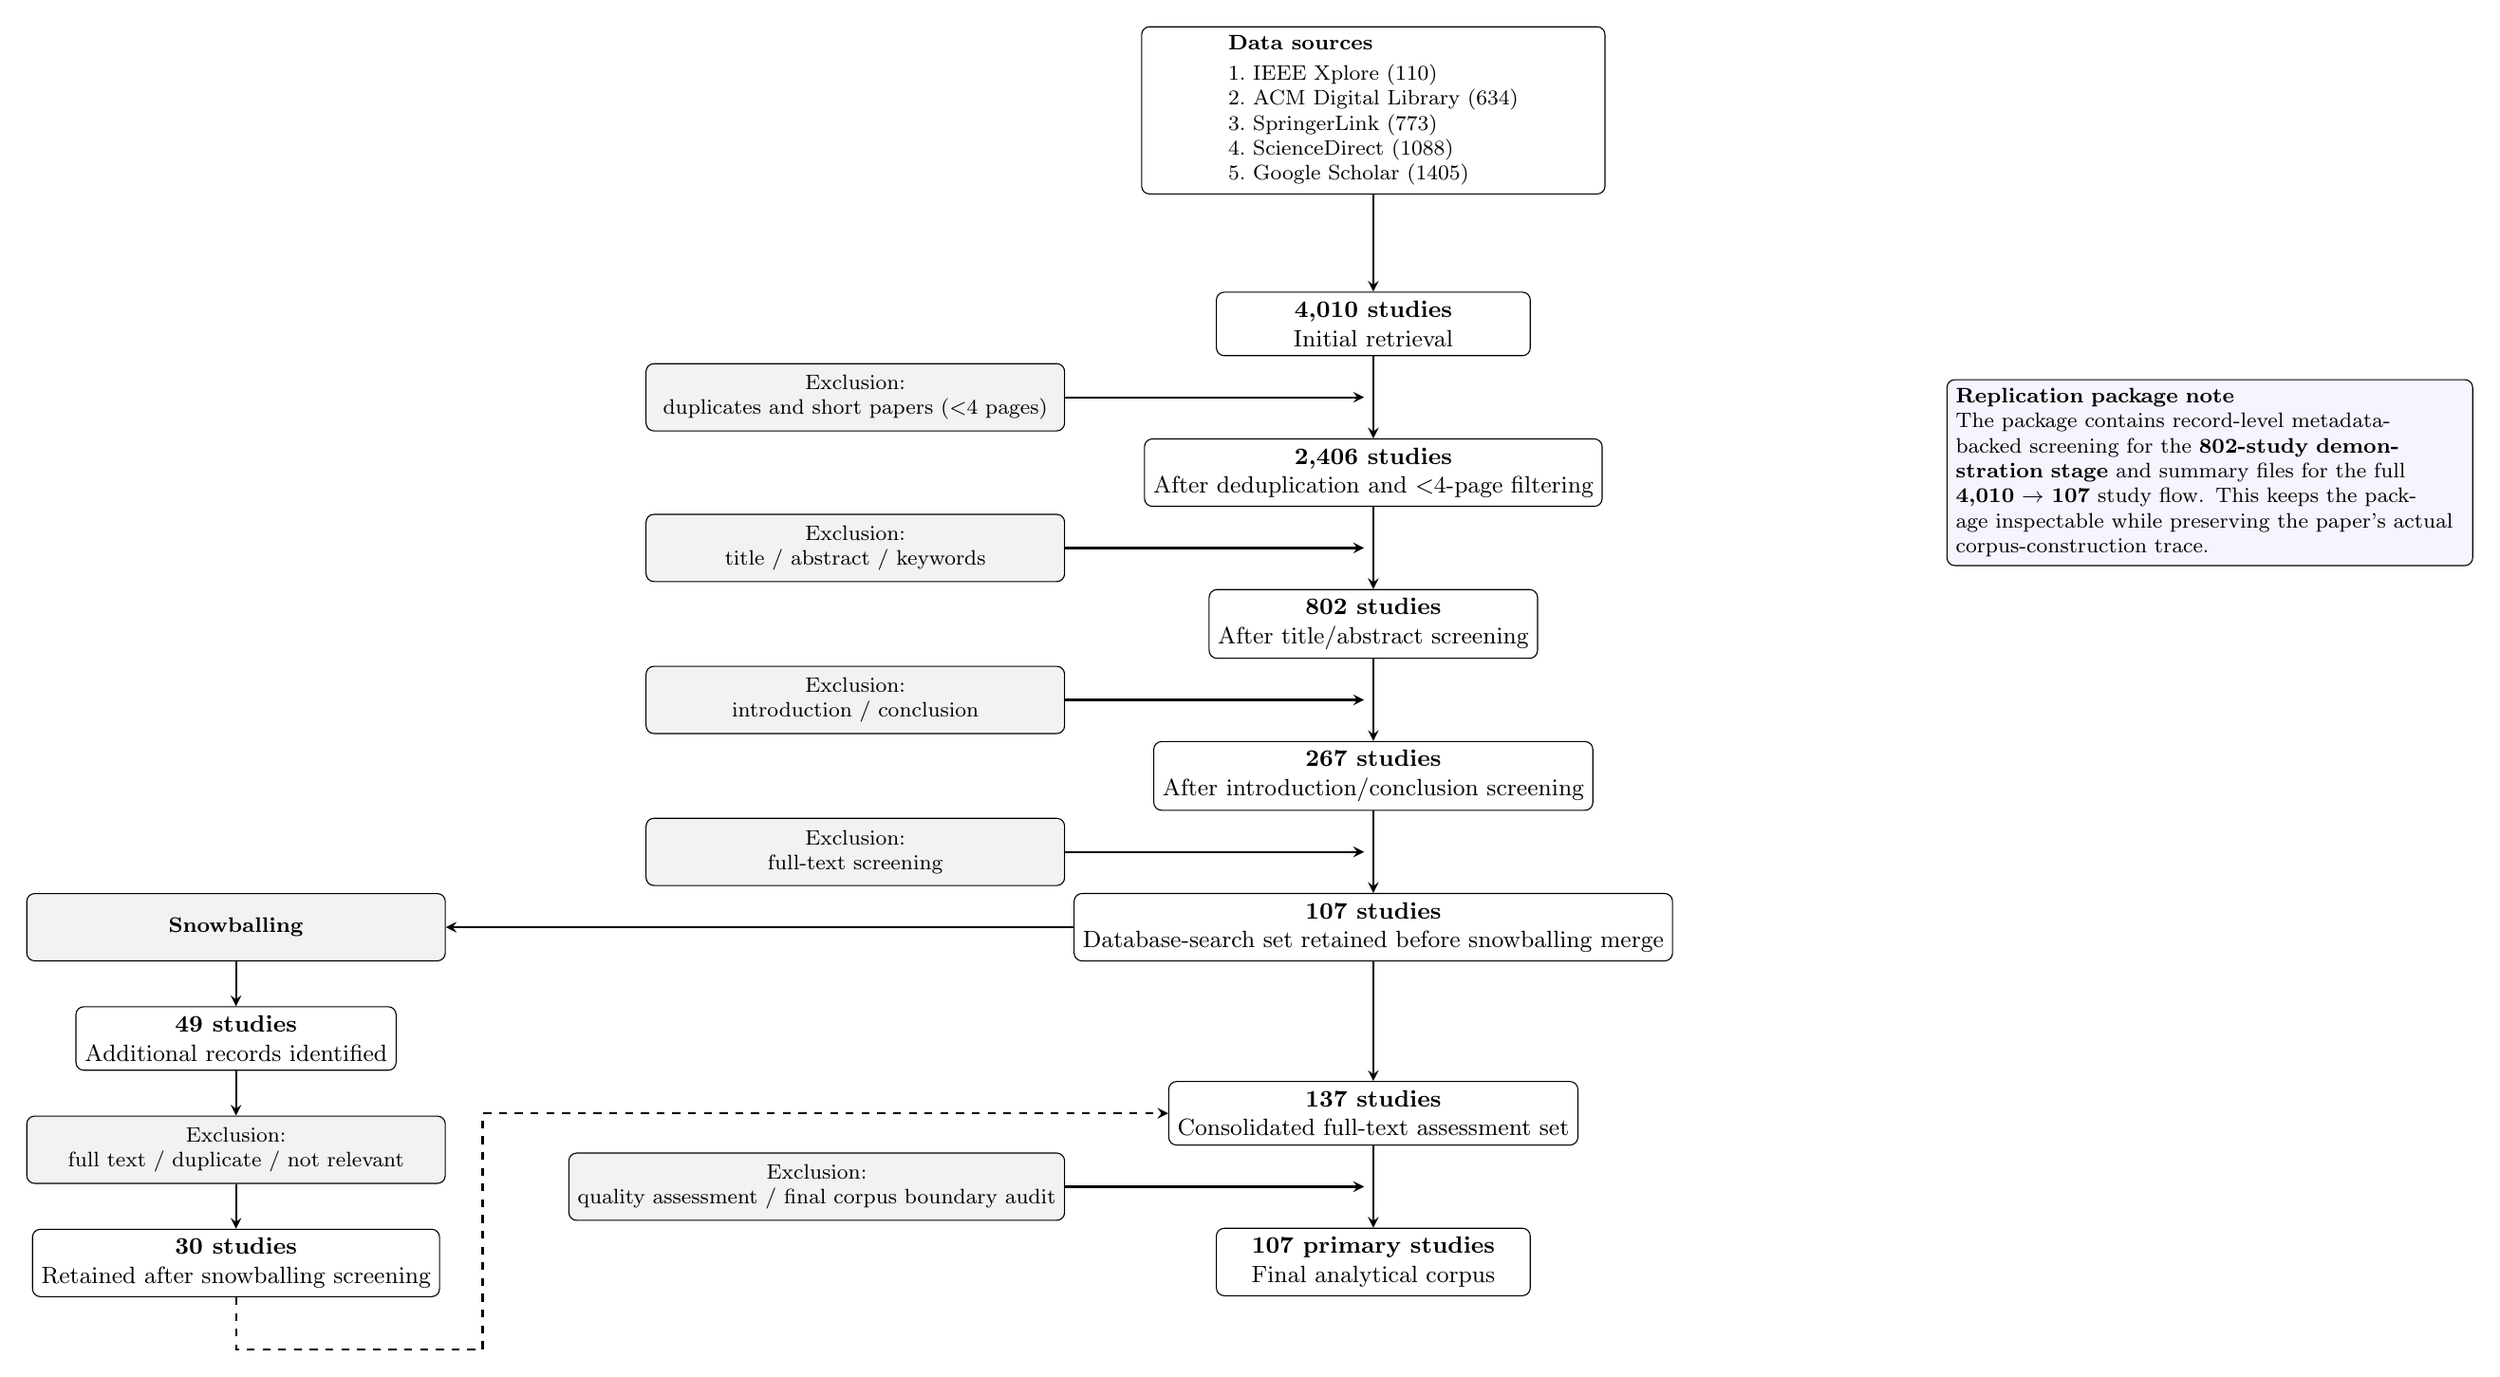
\begin{tikzpicture}[
    font=\small,
    >=stealth,
    line/.style={->, thick},
    dashedline/.style={->, thick, dashed},
    stage/.style={
        draw, rounded corners=3pt,
        minimum width=42mm,
        minimum height=8.5mm,
        align=center,
        fill=white
    },
    excl/.style={
        draw, rounded corners=3pt,
        fill=gray!10,
        minimum width=56mm,
        minimum height=9mm,
        align=center,
        font=\footnotesize
    },
    source/.style={
        draw, rounded corners=3pt,
        align=left,
        font=\footnotesize,
        minimum width=62mm,
        fill=white
    }
]

% Sources
\node[source] (sources) at (0,0) {%
\textbf{Data sources}\\[2pt]
1.\ IEEE Xplore (110)\\
2.\ ACM Digital Library (634)\\
3.\ SpringerLink (773)\\
4.\ ScienceDirect (1088)\\
5.\ Google Scholar (1405)
};

% Main vertical chain
\node[stage, below=13mm of sources] (s4010) {\textbf{4,010 studies}\\Initial retrieval};
\node[stage, below=11mm of s4010] (s2406) {\textbf{2,406 studies}\\After deduplication and $<$4-page filtering};
\node[stage, below=11mm of s2406] (s802)  {\textbf{802 studies}\\After title/abstract screening};
\node[stage, below=11mm of s802]  (s267)  {\textbf{267 studies}\\After introduction/conclusion screening};
\node[stage, below=11mm of s267]  (s107db) {\textbf{107 studies}\\Database-search set retained before snowballing merge};
\node[stage, below=16mm of s107db] (s137) {\textbf{137 studies}\\Consolidated full-text assessment set};
\node[stage, below=11mm of s137] (s107final) {\textbf{107 primary studies}\\Final analytical corpus};

% Main arrows
\draw[line] (sources.south) -- (s4010.north);
\draw[line] (s4010.south) -- (s2406.north);
\draw[line] (s2406.south) -- (s802.north);
\draw[line] (s802.south) -- (s267.north);
\draw[line] (s267.south) -- (s107db.north);
\draw[line] (s107db.south) -- (s137.north);
\draw[line] (s137.south) -- (s107final.north);

% midpoints
\path (s4010) -- (s2406) node[midway] (m1) {};
\path (s2406) -- (s802)  node[midway] (m2) {};
\path (s802)  -- (s267)  node[midway] (m3) {};
\path (s267)  -- (s107db) node[midway] (m4) {};
\path (s137)  -- (s107final) node[midway] (m5) {};

% Exclusion boxes
\node[excl, left=40mm of m1] (e1) {Exclusion:\\duplicates and short papers ($<$4 pages)};
\node[excl, left=40mm of m2] (e2) {Exclusion:\\title / abstract / keywords};
\node[excl, left=40mm of m3] (e3) {Exclusion:\\introduction / conclusion};
\node[excl, left=40mm of m4] (e4) {Exclusion:\\full-text screening};
\node[excl, left=40mm of m5] (e5) {Exclusion:\\quality assessment / final corpus boundary audit};

\draw[line] (e1.east) -- (m1.west);
\draw[line] (e2.east) -- (m2.west);
\draw[line] (e3.east) -- (m3.west);
\draw[line] (e4.east) -- (m4.west);
\draw[line] (e5.east) -- (m5.west);

% Snowballing branch
\node[excl, left=84mm of s107db] (snow) {\textbf{Snowballing}};
\node[stage, below=6mm of snow] (s49) {\textbf{49 studies}\\Additional records identified};
\node[excl, below=6mm of s49] (esnow) {Exclusion:\\full text / duplicate / not relevant};
\node[stage, below=6mm of esnow] (s30) {\textbf{30 studies}\\Retained after snowballing screening};

\draw[line] (s107db.west) -- ++(-10mm,0) |- (snow.east);
\draw[line] (snow.south) -- (s49.north);
\draw[line] (s49.south) -- (esnow.north);
\draw[line] (esnow.south) -- (s30.north);
\draw[dashedline] (s30.south) -- ++(0,-7mm) -- ++(33mm,0) |- (s137.west);

% demonstration note
\node[draw, rounded corners=3pt, fill=blue!4, align=left, font=\footnotesize, text width=68mm, anchor=west] at ($(s2406.east)+(46mm,0)$) {
\textbf{Replication package note}\\
The package contains record-level metadata-backed screening for the \textbf{802-study demonstration stage} and summary files for the full \textbf{4,010 $\rightarrow$ 107} study flow. This keeps the package inspectable while preserving the paper's actual corpus-construction trace.
};

\end{tikzpicture}%
}
\caption{Study selection and screening process for identifying primary studies. The record-level demonstration included in the replication package is centered on the 802 records retained after title/abstract screening, whereas the actual manuscript flow starts from 4,010 records and ends with 107 final primary studies.}
\label{fig:study-selection-replication-demo}
\end{figure}

\end{document}
